% Template for Cogsci submission with R Markdown

% Stuff changed from original Markdown PLOS Template
\documentclass[10pt, letterpaper]{article}

\usepackage{cogsci}
\usepackage{pslatex}
\usepackage{float}
\usepackage{caption}

% amsmath package, useful for mathematical formulas
\usepackage{amsmath}

% amssymb package, useful for mathematical symbols
\usepackage{amssymb}

% hyperref package, useful for hyperlinks
\usepackage{hyperref}

% graphicx package, useful for including eps and pdf graphics
% include graphics with the command \includegraphics
\usepackage{graphicx}

% Sweave(-like)
\usepackage{fancyvrb}
\DefineVerbatimEnvironment{Sinput}{Verbatim}{fontshape=sl}
\DefineVerbatimEnvironment{Soutput}{Verbatim}{}
\DefineVerbatimEnvironment{Scode}{Verbatim}{fontshape=sl}
\newenvironment{Schunk}{}{}
\DefineVerbatimEnvironment{Code}{Verbatim}{}
\DefineVerbatimEnvironment{CodeInput}{Verbatim}{fontshape=sl}
\DefineVerbatimEnvironment{CodeOutput}{Verbatim}{}
\newenvironment{CodeChunk}{}{}

% cite package, to clean up citations in the main text. Do not remove.
\usepackage{apacite}

% KM added 1/4/18 to allow control of blind submission
\cogscifinalcopy

\usepackage{color}

% Use doublespacing - comment out for single spacing
%\usepackage{setspace}
%\doublespacing


% % Text layout
% \topmargin 0.0cm
% \oddsidemargin 0.5cm
% \evensidemargin 0.5cm
% \textwidth 16cm
% \textheight 21cm

\title{The latent factor structure of child development}

\usepackage{bm}
\usepackage{booktabs}
\usepackage{longtable}
\usepackage{array}
\usepackage{multirow}
\usepackage{wrapfig}
\usepackage{float}
\usepackage{colortbl}
\usepackage{pdflscape}
\usepackage{tabu}
\usepackage{threeparttable}
\usepackage{threeparttablex}
\usepackage[normalem]{ulem}
\usepackage{makecell}
\usepackage{xcolor}

\author{Anonymous Cogsci Submission}

\begin{document}

\maketitle

\begin{abstract}
Hello

\textbf{Keywords:}
one; two;
\end{abstract}

\hypertarget{introduction}{%
\section{Introduction}\label{introduction}}

TO DO

\hypertarget{data}{%
\section{Data}\label{data}}

A child's development can be thought of as the set of developmental
milestones that they have reached at a particular point in time. This
conceptualization results in data with the same structure as the item
response data common to educational measurement. In education, item
response data is most typically students responding to test items (i.e.,
questions) and, in the dichotomous case, getting each question either
correct or incorrect. In the context of child development, the child is
the ``student,'' and each developmental milestone is the ``item.''

We use Kinedu, a Mexico-based child development app, as a source for
this type of data. When parents first start using the Kinedu app, they
are asked a series of questions about which developmental milestones
their child has reached. We consider the 1946 children between 2 and 55
months of age whose parents responded to all 414 of the developmental
milestones. Each developmental miletone on Kinedu is mapped to a
milestone group: physical, cognitive, linguistic, or social \&
emotional. Table \ref{tab:examples} shows the number of developmental
milestones in each group along with an example milestone translated to
English.

\begin{CodeChunk}
\begin{table}[!h]

\caption{\label{tab:examples}Developmental milestone groups and examples}
\centering
\fontsize{8}{10}\selectfont
\begin{tabular}[t]{l|r|l}
\hline
Group & Count & Milestone\\
\hline
Physical & 180 & Stands on their toes\\
\hline
Cognitive & 100 & Finds objects on the floor\\
\hline
Linguistic & 75 & Babbles to imitate conversations\\
\hline
Social \& Emotional & 59 & Complains when play is interrupted\\
\hline
\end{tabular}
\end{table}

\end{CodeChunk}

Figure \ref{fig:growth} shows the age (in months) and number of
developmental milestones for each child. At 12 months old, most children
have reached about 200 developmental milestones. At 24 months old, most
children have reached about 300 developmental milestones. Finally, at 48
months old, most children have reached about 375 of the 414
developmental milestones.

\begin{CodeChunk}
\begin{figure}[tb]
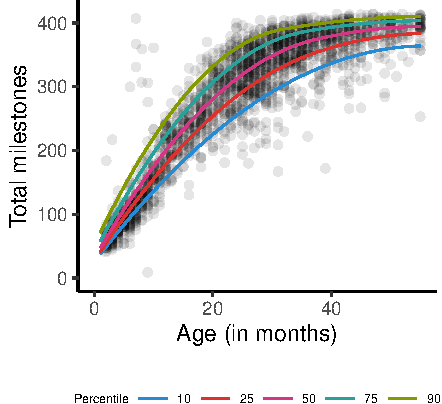
\includegraphics{figs/growth-1} \caption[Number of milestones by age]{Number of milestones by age}\label{fig:growth}
\end{figure}
\end{CodeChunk}

\hypertarget{empirical-assessment-of-the-dimensionality-of-child-development}{%
\section{Empirical assessment of the dimensionality of child
development}\label{empirical-assessment-of-the-dimensionality-of-child-development}}

We frame the assessment of the dimensionality of child development as a
model comparison question.

\hypertarget{models}{%
\subsection{Models}\label{models}}

Item response theory offers a suite of models with which to model item
response data. We adopt the notation used in Chalmers \& others (2012).
Let \(i = 1, \ldots, I\) represent the distinct children and
\(j = 1, \ldots, J\) the developmental milestones. The Kinedu item
response data is stored in a matrix, \(y\), where element \(y_{ij}\)
denotes if the \(i\)th child has or has not achieved the \(j\)th
developmental milestone as reported by their parent/guardian. Each model
represents the \(i\)th child's development using \(m\) latent factors
\(\boldsymbol{\theta}_{i}=(\theta_1, \ldots, \theta_m)\). The \(j\)th
milestone's discriminations (i.e.~slopes)
\(\boldsymbol{a_j}=(a_1, \dots, a_m)\) capture the latent factor
loadings onto that milestone.

We fit four two-parametric logistic (2PL) models where a child's
development is represented by \(m = 1, \ m = 2, \ m = 3,\) and \(m = 4\)
latent factors. According to the 2PL model, the probability of a child
having achieved a developmental milestone is \[
P(y_{ij} = 1 | \boldsymbol{\theta_i}, \boldsymbol{a_j}, b_j) = \sigma(\boldsymbol{a}_{j}^{\top}\boldsymbol{\theta_i} + b_j)
\] where \(b_j\) is the milestone easiness (i.e.~intercept) and
\(\sigma(x) = \frac{e^x}{e^x + 1}\) is the standard logistic function.

The 2PL models learn the latent factor structure entirely from the data,
making them exploratory. The bifactor model offers an alternative
specification where each milestone loads onto a general factor
\(\theta_0\) and a specific factor \(\theta_s\) (Cai, Yang, \& Hansen,
2011). The assignment of each developmental milestone to its specific
factor is an opportunity to specify the latent factor structure, making
the model confirmatory as opposed to exploratory. We map each milestone
to its specific factor according to the four developmental milestone
groups shown in Table \ref{tab:examples}. For the bifactor model, the
probability of a child having achieved a developmental milestone is \[
P(y_{ij} = 1 | \theta_0, \theta_s, a_0, a_s) = \sigma(a_0\theta_0 + a_s\theta_s + b_j).
\]

\hypertarget{model-comparison}{%
\subsection{Model comparison}\label{model-comparison}}

Model comparison in IRT typically uses information criterion such as AIC
and BIC (Maydeu-Olivares, 2013). However, these methods are not
guaranteed to work with modest sample sizes or misspecification
(McDonald \& Mok, 1995). Instead, we prefer a marginalized version of
cross-validation. In essence, we partition the data into folds based on
the children (i.e.~the rows of the item response matrix). Then for each
fold, we estimate the item parameters using all but that fold, and
calculate the likelihood of that fold by integrating over \(g(\theta)\).

Mathematically and following notation similar to Vehtari, Gelman, \&
Gabry (2017), we partition the data into \(K\) subsets \(y^{(k)}\) for
\(k = 1, \ldots, K\). Each model is fit separately to each training set
\(y^{(-k)}\) yielding item parameter estimates which we compactly denote
\(\Psi_j^{(-k)}\). The predictive (i.e.~out-of-sample) likelihood of
\(y^{(k)}\) is

\[
p(y^{(k)} | y^{(-k)}) = \prod_{i \in i^{(k)}}^{I} \int_\theta \prod_{j=1}^{J} \hat{\text{Pr}}(y_{ij}^{(k)} | \Psi_j^{(-k)}, \theta) g(\theta)d\theta.
\]

The ultimate quantity of interest for each model is the log predictive
likelihood for the entire item response matrix, which is defined as

\[
\text{lpl } y = \sum_{k = 1}^{K} \log p(y^{(k)} | y^{(-k)}).
\]

\hypertarget{results}{%
\subsection{Results}\label{results}}

Computing is done in R (R Core Team, 2019), model fitting in the R
package mirt (Chalmers \& others, 2012), and data
wrangling/visualization in the set of R packages known as the tidyverse
(Wickham, 2017).

\hypertarget{understanding-the-latent-factor-structure}{%
\subsection{Understanding the latent factor
structure}\label{understanding-the-latent-factor-structure}}

To understand each of the three factors in the best performing model, we
fit the model to the the full dataset. We then estimate the factor
loadings (i.e.~discriminations or slopes) using a varimax rotation. The
varimax rotation results in orthogonal and, therefore, more
interpretable factors (Kaiser, 1959). Figure \ref{fig:factorloadings}
shows the distribution of factor loadings for each group on each of the
three factors. The first factor is mainly cognitive and linguistic. The
second factor is a combination of each of the groups with the strongest
loadings on the physical and social \& emotional milestones. The third
mainly loads positively on linguistic milestones and negatively on
physical milestones.

\begin{CodeChunk}
\begin{figure}[tb]
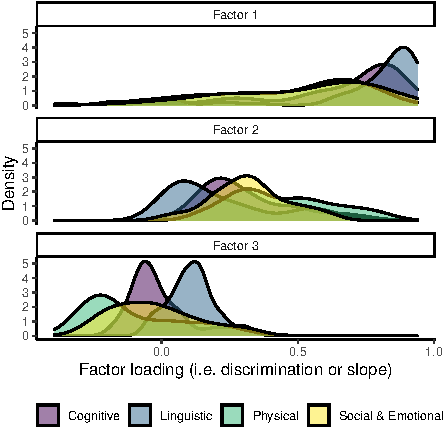
\includegraphics{figs/factorloadings-1} \caption[Factor loadings by group]{Factor loadings by group}\label{fig:factorloadings}
\end{figure}
\end{CodeChunk}

We also estimate the factor scores for each child using expected a
posteriori (EAP) with a three dimensional standard normal distribution
(Embretson \& Reise, 2013). Figure \ref{fig:factorscores} shows the
relationship between age and factor score for each factor. The first
factor, perhaps unsurprisingly, has a high correlation (r = 0.90) with
age. The second factor has a strong association with age from 2 to 16
months but thereafter is unrelated to age. By and large, the third
factor does not have any association with age.

\begin{CodeChunk}
\begin{figure}[tb]
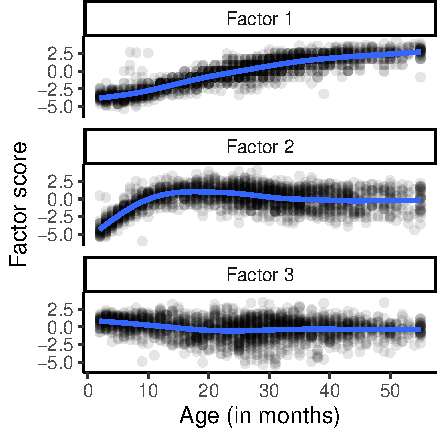
\includegraphics{figs/factorscores-1} \caption[The first factor is highly associated with age]{The first factor is highly associated with age}\label{fig:factorscores}
\end{figure}
\end{CodeChunk}

\hypertarget{acknowledgements}{%
\section{Acknowledgements}\label{acknowledgements}}

We'd like to thank Kinedu for providing the data that made this research
possible.

\hypertarget{references}{%
\section{References}\label{references}}

\setlength{\parindent}{-0.1in} 
\setlength{\leftskip}{0.125in}

\noindent

\hypertarget{refs}{}
\leavevmode\hypertarget{ref-cai2011generalized}{}%
Cai, L., Yang, J. S., \& Hansen, M. (2011). Generalized full-information
item bifactor analysis. \emph{Psychological Methods}, \emph{16}(3), 221.

\leavevmode\hypertarget{ref-chalmers2012mirt}{}%
Chalmers, R. P., \& others. (2012). Mirt: A multidimensional item
response theory package for the r environment. \emph{Journal of
Statistical Software}, \emph{48}(6), 1--29.

\leavevmode\hypertarget{ref-embretson2013item}{}%
Embretson, S. E., \& Reise, S. P. (2013). \emph{Item response theory}.
Psychology Press.

\leavevmode\hypertarget{ref-kaiser1959computer}{}%
Kaiser, H. F. (1959). Computer program for varimax rotation in factor
analysis. \emph{Educational and Psychological Measurement},
\emph{19}(3), 413--420.

\leavevmode\hypertarget{ref-maydeu2013goodness}{}%
Maydeu-Olivares, A. (2013). Goodness-of-fit assessment of item response
theory models. \emph{Measurement: Interdisciplinary Research and
Perspectives}, \emph{11}(3), 71--101.

\leavevmode\hypertarget{ref-mcdonald1995goodness}{}%
McDonald, R. P., \& Mok, M. M.-C. (1995). Goodness of fit in item
response models. \emph{Multivariate Behavioral Research}, \emph{30}(1),
23--40.

\leavevmode\hypertarget{ref-rcore}{}%
R Core Team. (2019). \emph{R: A language and environment for statistical
computing}. Vienna, Austria: R Foundation for Statistical Computing.
Retrieved from \url{https://www.R-project.org/}

\leavevmode\hypertarget{ref-vehtari2017practical}{}%
Vehtari, A., Gelman, A., \& Gabry, J. (2017). Practical bayesian model
evaluation using leave-one-out cross-validation and waic.
\emph{Statistics and Computing}, \emph{27}(5), 1413--1432.

\leavevmode\hypertarget{ref-tidy}{}%
Wickham, H. (2017). \emph{Tidyverse: Easily install and load the
'tidyverse'}. Retrieved from
\url{https://CRAN.R-project.org/package=tidyverse}

\bibliographystyle{apacite}


\end{document}
